%%%%%%%%%%%%%%%%%%%%%%%%%%%%%%%%%%%%%%%%%
% Daily Laboratory Book
% LaTeX Template
%
% This template has been downloaded from:
% http://www.latextemplates.com
%
% Original author:
% Frank Kuster (http://www.ctan.org/tex-archive/macros/latex/contrib/labbook/)
%
% Important note:
% This template requires the labbook.cls file to be in the same directory as the
% .tex file. The labbook.cls file provides the necessary structure to create the
% lab book.
%
% The \lipsum[#] commands throughout this template generate dummy text
% to fill the template out. These commands should all be removed when 
% writing lab book content.
%
% HOW TO USE THIS TEMPLATE 
% Each day in the lab consists of three main things:
%
% 1. LABDAY: The first thing to put is the \labday{} command with a date in 
% curly brackets, this will make a new page and put the date in big letters 
% at the top.
%
% 2. EXPERIMENT: Next you need to specify what experiment(s) you are 
% working on with an \experiment{} command with the experiment shorthand 
% in the curly brackets. The experiment shorthand is defined in the 
% 'DEFINITION OF EXPERIMENTS' section below, this means you can 
% say \experiment{pcr} and the actual text written to the PDF will be what 
% you set the 'pcr' experiment to be. If the experiment is a one off, you can 
% just write it in the bracket without creating a shorthand. Note: if you don't 
% want to have an experiment, just leave this out and it won't be printed.
%
% 3. CONTENT: Following the experiment is the content, i.e. what progress 
% you made on the experiment that day.
%
%%%%%%%%%%%%%%%%%%%%%%%%%%%%%%%%%%%%%%%%%

%----------------------------------------------------------------------------------------
%	PACKAGES AND OTHER DOCUMENT CONFIGURATIONS
%----------------------------------------------------------------------------------------

\documentclass[idxtotoc,hyperref,openany]{labbook} % 'openany' here removes the gap page between days, erase it to restore this gap; 'oneside' can also be added to remove the shift that odd pages have to the right for easier reading

\usepackage[ 
  backref=page,
  pdfpagelabels=true,
  plainpages=false,
  colorlinks=true,
  bookmarks=true,
  pdfview=FitB]{hyperref} % Required for the hyperlinks within the PDF
  
\usepackage{booktabs} % Required for the top and bottom rules in the table
\usepackage{float} % Required for specifying the exact location of a figure or table
\usepackage{graphicx} % Required for including images
\usepackage{lipsum} % Used for inserting dummy 'Lorem ipsum' text into the template

\newcommand{\HRule}{\rule{\linewidth}{0.5mm}} % Command to make the lines in the title page
\setlength\parindent{0pt} % Removes all indentation from paragraphs

\graphicspath{{../reports/figures/}} % Sets the path for all graphics, so only name is needed afterwards.

%----------------------------------------------------------------------------------------
%	DEFINITION OF EXPERIMENTS
%----------------------------------------------------------------------------------------

%\newexperiment{example}{This is an example experiment}
%\newexperiment{example2}{This is another example experiment}
\newexperiment{First steps}{}
\newexperiment{Data cleaning}{}
\newexperiment{table}{This shows a sample table}
%\newexperiment{shorthand}{Description of the experiment}

%---------------------------------------------------------------------------------------

\begin{document}

%----------------------------------------------------------------------------------------
%	TITLE PAGE
%----------------------------------------------------------------------------------------

\frontmatter % Use Roman numerals for page numbers
\title{
\begin{center}
\HRule \\[0.4cm]
{\Huge \bfseries Lab Book \\[0.5cm] \Large Machine Learning}\\[0.4cm] % Degree
\HRule \\[1.5cm]
\end{center}
}
\author{\Huge C\'ordoba Romero, Javier \\ \Huge Corroto Mart\'in, Juan Jos\'e \\ \Huge Guerrero del Pozo, \'Alvaro \\ \\[2cm]} % Your name and email address
\date{Beginning 10 October 2018} % Beginning date
\maketitle

\tableofcontents

\mainmatter % Use Arabic numerals for page numbers

%----------------------------------------------------------------------------------------
%	LAB BOOK CONTENTS
%----------------------------------------------------------------------------------------

% Blank template to use for new days:

%\labday{Day, Date Month Year}

%\experiment{}

%Text

%-----------------------------------------

%\experiment{}

%Text

%----------------------------------------------------------------------------------------

\labday{Wednesday, 10 October 2018}
\experiment{First steps}

Done by Juan Jos\'e Corroto, Javier C\'ordoba and \'Alvaro Guerrero\\

We've initialized the repo with \texttt{coookiecutter} directory structure and learnt the purpose of each directory.
We've also learnt how to work with \texttt{pandas}, read and write a csv and how to work with spyder.

%----------------------------------------------------------------------------------------

\experiment{Data cleaning}

We've picked the data of only the first day, we've done this by looking at the raw data and looking at the column \textit{"TimeStemp"}.

Then we've deleted the \textit{UUID, Version} and \textit{TimeStemp} columns because they were non-numerical values.

Then we've tried deleting the rows that had \textit{NaN} values, and we ended up deleting the whole dataframe. So, after scanning the dataframe, we have realized that the columns 
\begin{enumerate}
\item \textit{RotationVector\_cosThetaOver2\_MEAN}
\item \textit{RotationVector\_cosThetaOver2\_MEDIAN}
\item \textit{RotationVector\_cosThetaOver2\_MIDDLE\_SAMPLE}
\end{enumerate}
Had all their values as \textit{Nan}.
\\
After eliminating these 3 columns, we proceeded as before: we eliminated those rows that had \textit{NaN} values and deleted 2 rows.

Then we saved this new data as processed data in its corresponding folder: data/interim/.

%----------------------------------------------------------------------------------------


\labday{Wednesday, 17 October 2018}
\experiment{Feature Selection}

Done by Juan Jos\'e Corroto, Javier C\'ordoba and \'Alvaro Guerrero\\

First, we have modified how we pick the first day data: instead of getting the 2038 first rows, we convert the \textit{'Timestemp'} to days and choosing the day 28 (the first one).\\

In addition to the columns dropped the last week, we have also dropped \textit{UUID}. Then every \textit{FFT} and \textit{Middle Sample} rows have been dropped too.\\

We have chosen just two sensors to do an initial exploration: \textbf{Accelerometer} and \textbf{Linear acceleration}. The purpose is to try and explore the data related to the movement of the phone.\\
So, we create a new dataframe with only \textit{Acelerometer} and \textit{Linear Aceleration}. Finally, we drop \textit{Covariances}, as we don't think they will be useful cause they are calculated as the relation \textit{2-by-2} of the axis.

\experiment{Visualization - Clustering}

We then calculate the \textit{PCA} with an \textit{explained\_variance\_ratio} of \textbf{0.78} and \textbf{0.14}, which is a very good representation of the original 18 features we were studying.

With this results, we plot a \textit{scatterplot} to visualize it(Figure \ref{data plot 1}).

\begin{figure}[h]
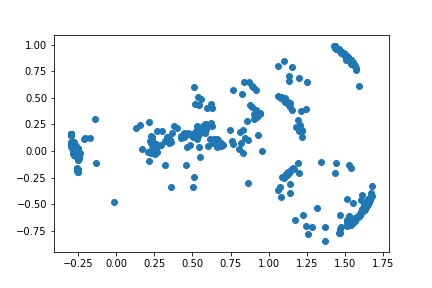
\includegraphics[width=0.9\linewidth]{PCA_Plot_Accelerometer_Day1.png}
\setlength\belowcaptionskip{-10pt}
\caption{Plot of the data after PCA}
\label{data plot 1}
\end{figure}



After that we run the \textit{k-means} algorithm with different number of centroids and print the \textit{silhouette} and \textit{distortion}. We initialize the centroids using the \textit{K-means++}algorithm as well. You can see the measurements of distortion and silhouette of KMeans with different number of centroids in figures \ref{K-means distortion 1} and \ref{K-means silhouette 1} respectively.\\


\begin{figure}[h]
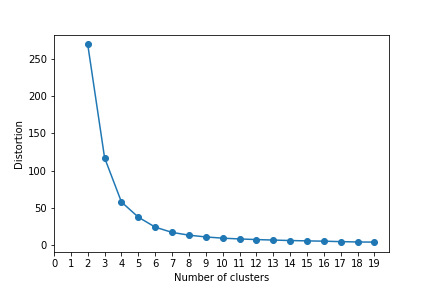
\includegraphics[width=0.9\linewidth]{KMeans_Distortion_Accelerometer_Day1.png}
\setlength\belowcaptionskip{-10pt}
\caption{Distortion of K-means with different number of centroids}
\label{K-means distortion 1}
\end{figure}

\begin{figure}[h]
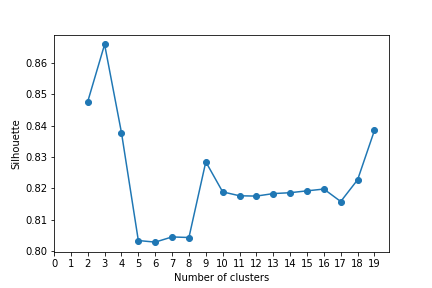
\includegraphics[width=0.9\linewidth]{KMeans_Silhouette_Accelerometer_Day1.png}
\setlength\belowcaptionskip{-10pt}
\caption{Silhouette of K-means with different number of centroids}
\label{K-means silhouette 1}
\end{figure}
By looking at the plots, we have decided to choose \textbf{4} as the final number of centroids.\\

Finally, we run the \textit{k-means} algorithm with said number of centroids and plot the results, each cluster having a different color, and the centroids being colored in red.\\

\begin{figure}[h]
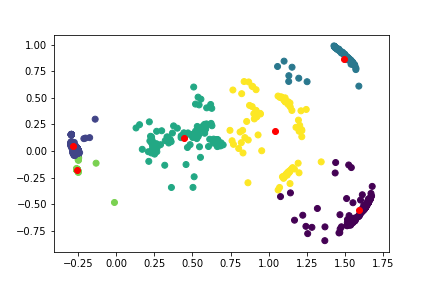
\includegraphics[width=0.9\linewidth]{KMeans_Plot_Accelerometer_Day1.png}
\setlength\belowcaptionskip{-10pt}
\caption{Plot of the data after K-means (centroids in red)}
\label{K-Means plot 1}
\end{figure}


Before trying to get meaning from the clusters, we have decided to repeat this experiment by doing some exploration on the features.


%----------------------------------------------------------------------------------------

\labday{Friday, 26 October 2018}
\experiment{Feature Selection done well}

Done by Juan Jos\'e Corroto.

We have repeated the same process as before: pick the day 1 data from the whole database, but this time, we are going to perform some analysis on the features in order to remove those features that gives us less value due to redundancy, instead of removing some columns randomly.
First, we still remove all columns that have to do with the \textit{Fast Fourier transform}, since we don't know how it works and we can not extract knowledge from them. The same with the \textit{Middle Sample} columns.
After that we remove \textit{NaN} columns and rows as we were doing proviously.\\

Now we are going to see the correlation between the features:

\begin{figure}[h]
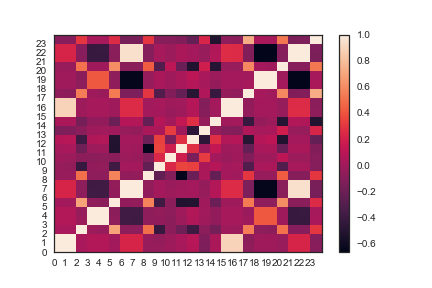
\includegraphics[width=0.9\linewidth]{Features_CorrelationMatrix_preDrop_Day1.png}
\setlength\belowcaptionskip{-10pt}
\caption{Correlation of the 24 features we now have}
\label{Correlation predrop}
\end{figure}

We can see some variables with a very high correlation in figure \ref{Correlation predrop}. There are some couple of features with a correlation near to 1 (The maximum value), like features 0 and 1, or 21 and 22. This features are the mean and median values of every axis, so we remove all median values from our features. \\

Having a very similar median and mean values gives us some information: The mean of a value is an stimator strongly affected by outliers, while the median is not. If the median and the mean have similar values, this means little ammount of outliers in our data (It does not mean they are non existent).\\

From the correlation matrix we can also see some features with a very big correlation: the mean values of each axis between both sensors. This means the value of x for the Accelerometer and the LinearAcceleration are highly correlated, so we remove one of those (In this case, the value of the Accelerometer is dropped). The result can be seen in Figure \ref{Correlation postdrop}.

\begin{figure}[h]
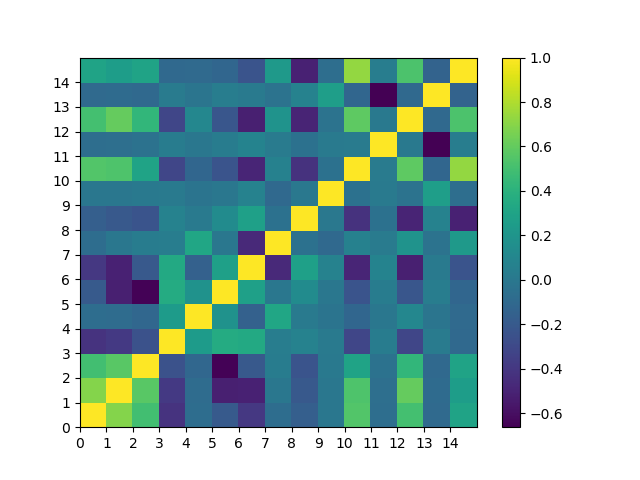
\includegraphics[width=0.9\linewidth]{Features_CorrelationMatrix_postDrop_Day1.png}
\setlength\belowcaptionskip{-10pt}
\caption{Correlation of the 15 features we now have after removing some}
\label{Correlation postdrop}
\end{figure}


There are a couple of features that are still highly correlated: The variances of the accelerometer, but this correlation is not high enough to remove them straight up, so we are going to use hierarchical clustering to see if we can extract more information. As seen in the Figure \ref{Clustering features}, there are some clusters of features, but the most similar ones are features 0, 1, 2 and 12. Those are the variances of the accelerometer. These are the features we were looking for, therefore, we can use only one of them.

\begin{figure}[h]
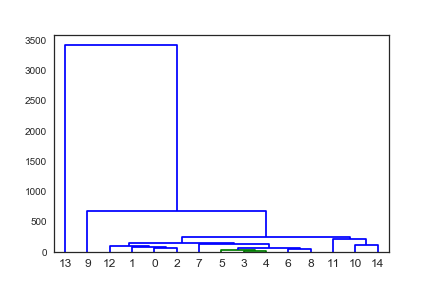
\includegraphics[width=0.9\linewidth]{Features_Dendogram_Day1.png}
\setlength\belowcaptionskip{-10pt}
\caption{Features dendogram}
\label{Clustering features}
\end{figure}

\experiment{Repeating the process}

Done by Juan Jos\'e Corroto.

With our new dataset finished from the previous experiment, we are going to repeat the process of our last day. First we apply PCA with an \textit{explained\_variance\_ratio} of \textbf{0.76} and \textbf{0.14}. This ratio is very similar to the one we had in the previous iteration, and pretty good considering we have removed features that were highly correlated. 
\\

\begin{figure}[h]
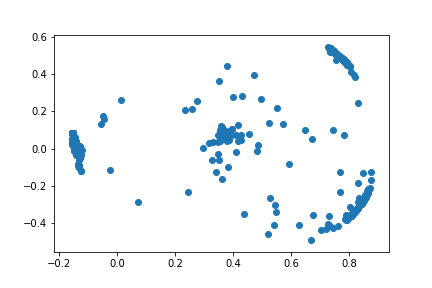
\includegraphics[width=0.9\linewidth]{PCA_Plot_Accelerometer_Day1_Selected.png}
\setlength\belowcaptionskip{-10pt}
\caption{Plot of the data after PCA}
\label{data plot 1 Selected}
\end{figure}

The data is plotted in Figure \ref{data plot 1 Selected}, and we can see some differences with respect to the plot we had in the previous day.
\\
We run K-means several times again. We get very good values of Distortion and Silhouette again, thought this time they are even better for 4 clusters, so we select again this number of clusters and run K-means, with the plotted results shown in Figure \ref{K-Means plot 1 Selected}.


\begin{figure}[h]
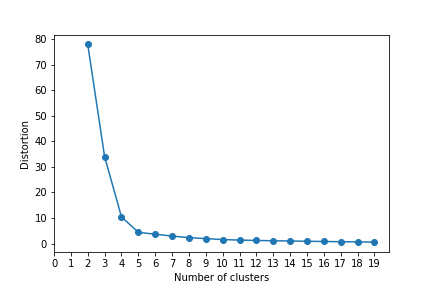
\includegraphics[width=0.9\linewidth]{KMeans_Distortion_Accelerometer_Day1_Selected.png}
\setlength\belowcaptionskip{-10pt}
\caption{Distortion of K-means with different number of centroids}
\label{K-means distortion 1 Selected}
\end{figure}

\begin{figure}[h]
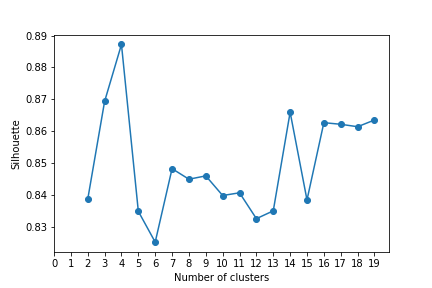
\includegraphics[width=0.9\linewidth]{KMeans_Silhouette_Accelerometer_Day1_Selected.png}
\setlength\belowcaptionskip{-10pt}
\caption{Silhouette of K-means with different number of centroids}
\label{K-means silhouette 1 Selected}
\end{figure}

\begin{figure}[h]
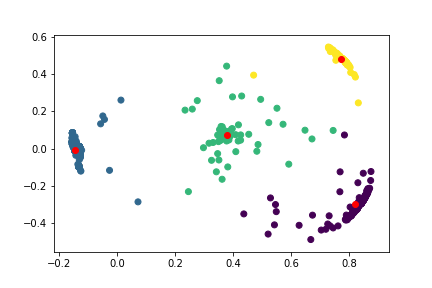
\includegraphics[width=0.9\linewidth]{KMeans_Plot_Accelerometer_Day1_Selected.png}
\setlength\belowcaptionskip{-10pt}
\caption{Plot of the data after K-means (centroids in red)}
\label{K-Means plot 1 Selected}
\end{figure}


%----------------------------------------------------------------------------------------

\labday{Saturday, 27 October 2018}
\experiment{Using other sensors}

Done by \'Alvaro Guerrero del Pozo.

In this experiment, we have used what we have learnt until now, this time applied to other sensors. Again, we load the dataset, but just keep the data of the first day. Then, we drop any column that contains no information (i.e is null) and rows with null values. Then, we just keep columns related to \textit{GyroscopeStat} and \textit{RotationVector}

As before, we now plot correlations between features:

\begin{figure}[h]
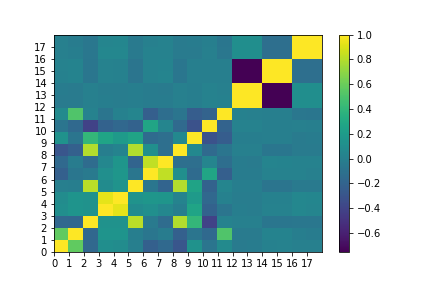
\includegraphics[width=0.9\linewidth]{2710/Features_CorrelationMatrix_preDrop.png}
\setlength\belowcaptionskip{-10pt}
\caption{Correlation of the 18 features}
\label{Correlation Predrop Gyroscope}
\end{figure}


As expected, \textit{Mean} and \textit{Median} values of each axis, of both sensors are highly correlated, so we can safely drop one of them, as the only add redundant informacion. We choose to remove \textit{Median} values. But, there is an exception: X axis of the \textit{Gyroscope}. The correlation between \textit{Mean} and \textit{Median} isn't high enough, so we don't remove any of them.
Also, we can see that there is a surprisingly high (inverse) correlation between \textit{Y Mean} and \textit{X Mean} of the \textit{Rotation Vector}.\\\\\\
It's not as high as other values (most of the previous ones had a correlation of near to 1), but still, with a correlation of around \textbf{-0.75}, we have decided to remove \textit{Y Mean}.

As a result, we are left with 12 features, whose correlations can be seen in the next figure:

\begin{figure}[h]
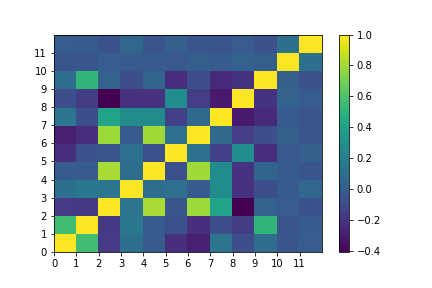
\includegraphics[width=0.9\linewidth]{2710/Features_CorrelationMatrix_postDrop.png}
\setlength\belowcaptionskip{-10pt}
\caption{Correlation of the 12 features}
\label{Correlation Postdrop Gyroscope}
\end{figure}

\clearpage
After that, we plot the dendogram of the features (Figure \ref{Dendogram Gyroscope}).

\begin{figure}[h]
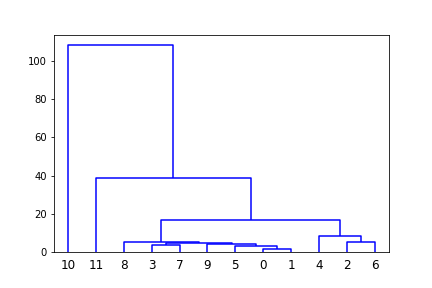
\includegraphics[width=0.9\linewidth]{2710/Features_Dendogram.png}
\setlength\belowcaptionskip{-10pt}
\caption{Dendogram}
\label{Dendogram Gyroscope}
\end{figure}

As we can see, the most similar features are the \textit{Variances} of the three axis of the gyroscope (at, the left, in green color), so we drop two of them, as they don't add much informacion, and keep only \textit{GyroscopeStat\_x\_VAR}. 
The next more similar features (right, red color), are \textit{GyroscopeStat\_x\_MEDIAN} and \textit{GyroscopeStat\_COV\_z\_x}, wich is something we were expecting, due to the influence of the x axis of the \textit{Gyroscope} in both features. Due to this fact, we don't consider this features similar enough so one of them gets removed, so we keep both.

\clearpage
Now that we have our data only with the features that are considered relevant, we proceed to visualize the data, by using \textit{k-means}.\\

First, we apply PCA, and obtain an \textit{explained\_variance\_ratio} of \textbf{0.825} and \textbf{0.130}. It's a high result, so we expect to obtain a good visualization. The plot of PCA is:

\begin{figure}[h]
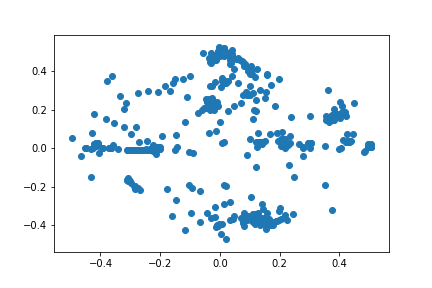
\includegraphics[width=0.9\linewidth]{2710/PCA_Plot_Gyroscope.png}
\setlength\belowcaptionskip{-10pt}
\caption{Plot of the data after PCA}
\label{Plot Gyroscope}
\end{figure}  

\textit{  }\\\\\\\
After that, we run \textit{k-means} several times, from 2 to 20 \textit{centroids} and plot the Distortion \ref{Distortion Gyroscope} and Silhouette \ref{Silhouettes Gyroscope}.

\begin{figure}[h]
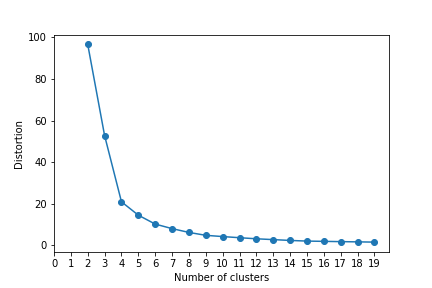
\includegraphics[width=0.9\linewidth]{2710/KMeans_Distortion_Gyroscope.png}
\setlength\belowcaptionskip{-10pt}
\caption{Distortion}
\label{Distortion Gyroscope}
\end{figure}  

\begin{figure}[h]
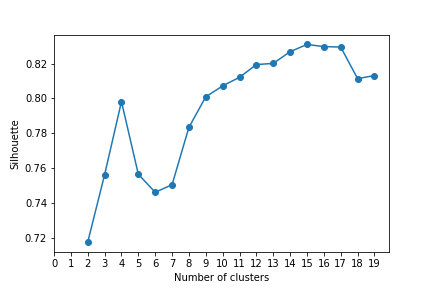
\includegraphics[width=0.9\linewidth]{2710/KMeans_Silhouttes_Gyroscope.png}
\setlength\belowcaptionskip{-10pt}
\caption{Silhouettes}
\label{Silhouettes Gyroscope}
\end{figure}  

\clearpage

We choose 4 as the best number of \textit{centroids}, as there is a maximun in the \textit{silhouette}, and the \textit{distortion} is low. The resulting plot is shown below.

\begin{figure}[h]
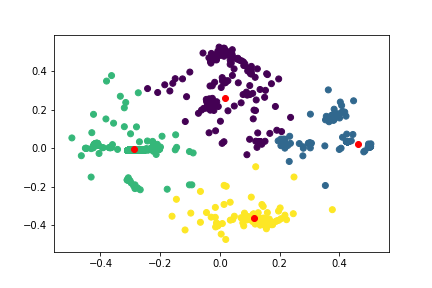
\includegraphics[width=0.9\linewidth]{2710/KMeans_Plot_Gyroscope.png}
\setlength\belowcaptionskip{-10pt}
\caption{Plot of the data after K-means (centroids in red)}
\label{K-Means Gyroscope}
\end{figure}

As we can see, the centroids have been placed where there are higher concentrain of points, but there is a decent amount of points that would be assigned to the neightbour cluster, should the centroids change slightly. Is a matter for another experiment to interpret this results, and decide wether they are good enough or not.

%----------------------------------------------------------------------------------------

\labday{Tuesday, 30 October 2018}

\experiment{Selecting different data}
The aim of this experiment is to select data from a different day, to see if it is significantly different than that of the first day. So, we are going to repeat the process of studying the \textit{Acceleromenter} and \textit{Linear Acceleration} variables.
\\

The first thing to do is to remove all the features we can not use: as before, we remove the timestamp and the non-numerical values, and also the features that have something to do with the \textit{First Fourier Transform}. After that we study the correlation between variables.

\begin{figure}[h]
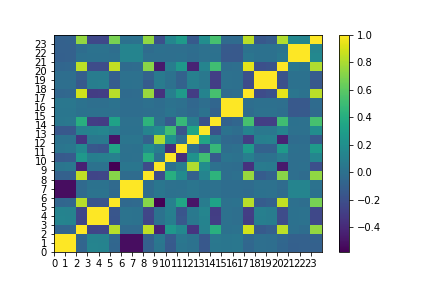
\includegraphics[width=0.9\linewidth]{Features_CorrelationMatrix_preDrop_Day2.png}
\setlength\belowcaptionskip{-10pt}
\caption{Correlation of the 24 features we have}
\label{Correlation predrop2}
\end{figure}

\begin{figure}[h]
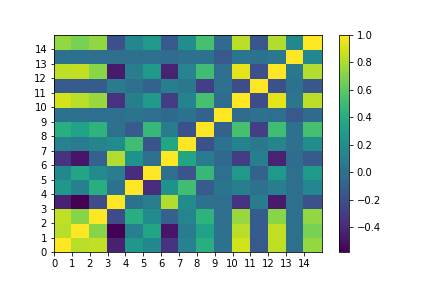
\includegraphics[width=0.9\linewidth]{Features_CorrelationMatrix_postDrop_Day2.png}
\setlength\belowcaptionskip{-10pt}
\caption{Correlation of the 15 features we now have after removing some}
\label{Correlation postdrop2}
\end{figure}

\begin{figure}[h]
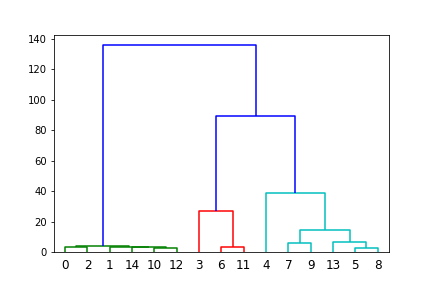
\includegraphics[width=0.9\linewidth]{Features_Dendogram_Day2.png}
\setlength\belowcaptionskip{-10pt}
\caption{Features dendogram}
\label{Clustering features2}
\end{figure}

As we can see in figures \ref{Correlation predrop2}, \ref{Correlation postdrop2} and \ref{Clustering features2}, the situation is very similar: The mean and median of every sensor is highly correlated, and the variances of the accelerometer are highly correlated but not high enough too discard them. But when making the clustering we have proof enough that their information is very similar and we discard them as well, leaving us with the same 12 features we had on the previous experiment.

We are now going to plot the data, as seen in figure \ref{data plot 2 Selected}. For that we have to, of course, apply PCA. In this case, the \textit{explained\_variance\_ratio} is a little lower: \textbf{0.51134397} and \textbf{0.17562308}. This can be explained because we have almost double the data as before. Anyways, it is still high enough to have a good representation of the data.

\begin{figure}[h]
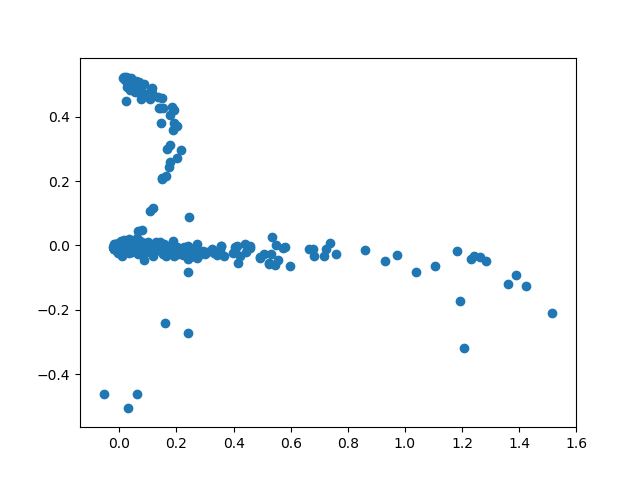
\includegraphics[width=0.9\linewidth]{PCA_Plot_Accelerometer_Day2_Selected.png}
\setlength\belowcaptionskip{-10pt}
\caption{Plot of the data after PCA}
\label{data plot 2 Selected}
\end{figure}

The next step is to do some clustering to the data. As before, we are going to use \textit{K-means}, and we are also going to use the elbow method to see the best number of clusters.


\begin{figure}[h]
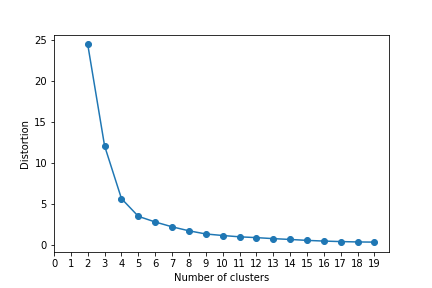
\includegraphics[width=0.9\linewidth]{KMeans_Distortion_Accelerometer_Day2_Selected.png}
\setlength\belowcaptionskip{-10pt}
\caption{Distortion of K-means with different number of centroids}
\label{K-means distortion 2 Selected}
\end{figure}

\begin{figure}[h]
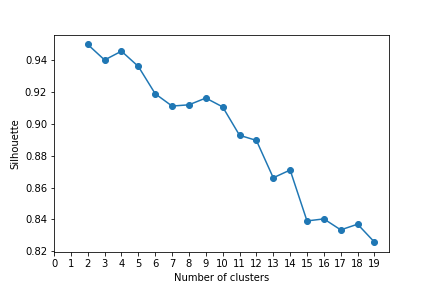
\includegraphics[width=0.9\linewidth]{KMeans_Silhouette_Accelerometer_Day2_Selected.png}
\setlength\belowcaptionskip{-10pt}
\caption{Silhouette of K-means with different number of centroids}
\label{K-means silhouette 2 Selected}
\end{figure}

\begin{figure}[h]
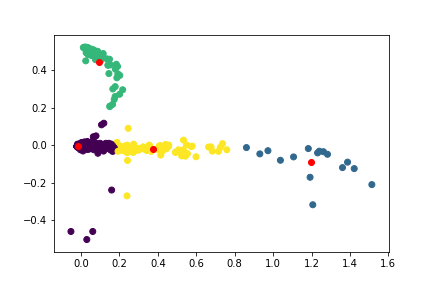
\includegraphics[width=0.9\linewidth]{KMeans_Plot_Accelerometer_Day2_Selected.png}
\setlength\belowcaptionskip{-10pt}
\caption{Plot of the data after K-means (centroids in red)}
\label{K-Means plot 2 Selected}
\end{figure}

In figures \ref{K-means distortion 2 Selected} and \ref{K-means silhouette 2 Selected} we can infere that, again, a good number of clusters is 4. In Figure \ref{K-Means plot 2 Selected} we can see a plot of the data after clustering. The data looks a lot different than that of the first day, and the clusters seem less defined even. Maybe we should try a different cluster algorithm than K-means?

%----------------------------------------------------------------------------------------

\labday{Thursday, 31 October 2018}

\experiment{Density based clustering: DBSCAN}
After clustering both our \textit{Accelerometer} and \textit{Gyroscope} data with a traditional approach, that is, KMeans.

We are going to cluster it using a density based approach with the use of the \texttt{DBSCAN} algorithm. The settings used (\textit{epsilon} and \textit{minPts}) have been tuned manually to get the best results.


\begin{figure}[h]
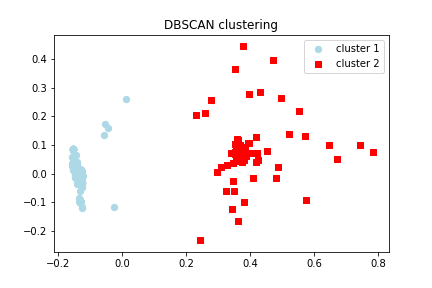
\includegraphics[width=0.9\linewidth]{DBSCAN_Plot_Accelerometer_Day1.png}
\setlength\belowcaptionskip{-10pt}
\caption{Accelerometer Day1 after clustering with DBSCAN}
\label{DBSCAN AccelerometerDay1}
\end{figure}

\begin{figure}[h]
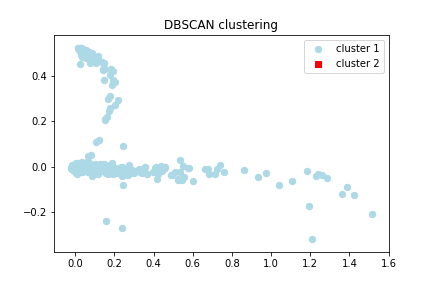
\includegraphics[width=0.9\linewidth]{DBSCAN_Plot_Accelerometer_Day2.png}
\setlength\belowcaptionskip{-10pt}
\caption{Accelerometer Day2 after clustering with DBSCAN}
\label{DBSCAN AccelerometerDay2}
\end{figure}

\begin{figure}[h]
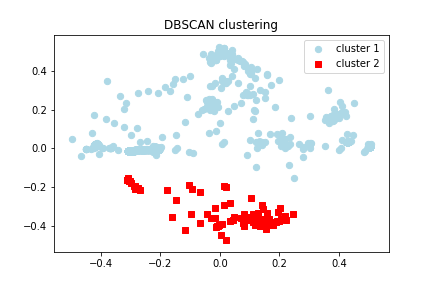
\includegraphics[width=0.9\linewidth]{DBSCAN_Plot_Gyroscope.png}
\setlength\belowcaptionskip{-10pt}
\caption{Gyroscope after clustering with DBSCAN}
\label{DBSCAN Gyroscope}
\end{figure}

As we can see in figures \ref{DBSCAN AccelerometerDay1}, and \ref{DBSCAN Gyroscope} DBSCAN is not able to correctly cluster the data because it divides the plot in half and also loses some data points. However, in figure \ref{DBSCAN AccelerometerDay2} we can clearly see that the data is now clustered correctly, it distinguishes between two clearly differentiated groups.
 
Because of this we are only going to use \texttt{DBSCAN} based clustering in the Accelerometer Day2.


\experiment{Density based clustering: Local Outlier Factor (LOF)}
After our first approach with density based clustering using DBSCAN we are now going to detect outliers with another density based clustering approach: \textit{Local Outlier Factor}.
\\

This algorithm gives each data point an outlier score, as opposed to other algorithms that give a binary score (outlier or not outlier). So, in order to get a set of outliers we select only the data points that are in the 99 percentile of outlier score


\begin{figure}[h]
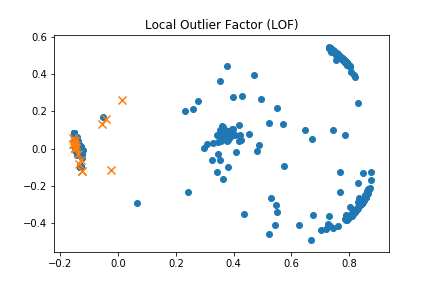
\includegraphics[width=0.9\linewidth]{LOF_Plot_Accelerometer_Day1.png}
\setlength\belowcaptionskip{-10pt}
\caption{Accelerometer Day1 LOF Outliers}
\label{LOF AccelerometerDay1}
\end{figure}

\begin{figure}[h]
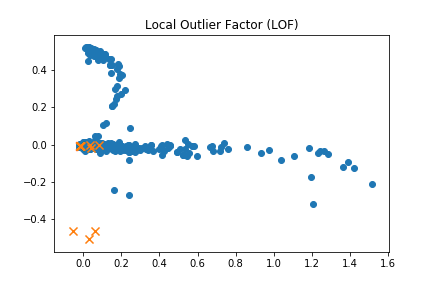
\includegraphics[width=0.9\linewidth]{LOF_Plot_Accelerometer_Day2.png}
\setlength\belowcaptionskip{-10pt}
\caption{Accelerometer Day2 LOF Outliers}
\label{LOF AccelerometerDay2}
\end{figure}

\begin{figure}[h]
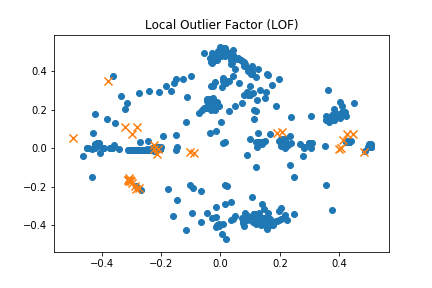
\includegraphics[width=0.9\linewidth]{LOF_Plot_Gyroscope.png}
\setlength\belowcaptionskip{-10pt}
\caption{Gyroscope LOF Outliers}
\label{LOF Gyroscope}
\end{figure}

As we can see in figures \ref{LOF AccelerometerDay1}, \ref{LOF AccelerometerDay2} and \ref{LOF Gyroscope} the outliers (marked with an \textbf{x}) are not outliers in the plot. 

The reason for this is that the data that is represented is the result of applying PCA to the original data, a consequence of this is that the data does not represent the shape nor the values that it originally had.

%----------------------------------------------------------------------------------------
\labday{Thursday, 1st November 2018}
\experiment{Interpreting the results: Gyroscope}

After all the previous experiments, the only remaining work is interpreting the results. In this section, we will interpret the results of the Gyroscope. \\
We are going to focus on the \textit{Rotation\_Vector}. The first part is understanding how the three axis of this sensor work.

\begin{figure}[h]
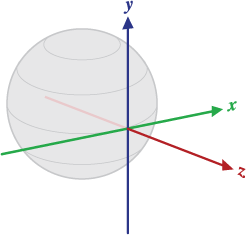
\includegraphics[width=0.9\linewidth]{sensors/rotationvector_axis_globe.png}
\setlength\belowcaptionskip{-10pt}
\caption{Rotation Vector Axis Globe}
\label{Rotation Vector Axis Globe}
\end{figure}

\clearpage
By looking at the image, we can interpret that the z axis is perpendicular to the phone screen, the y axis is parallel to the phone's longest side, and x axis is perpendicular to both of them.\\
The sensors \textit{should} give a result of 0 when te phone is laying in an \textbf{horizontal surface}.\\\\
The next thing we do is plotting the results of the clustering along with the measures of the sensors. We'll use \textit{seaborn} library for that.

\begin{figure}[h]
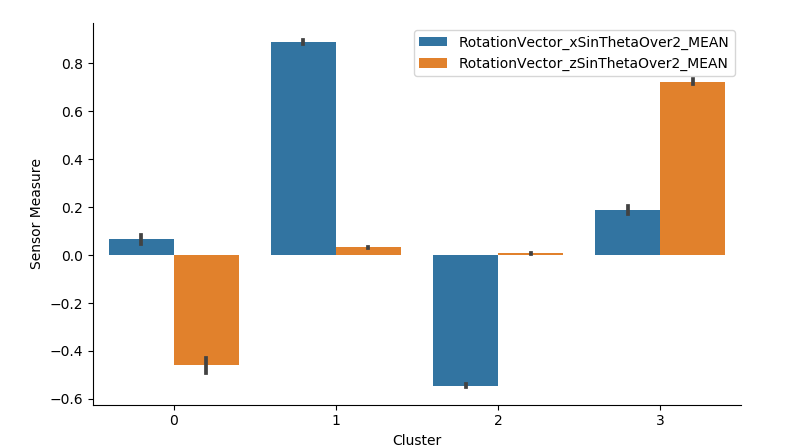
\includegraphics[width=0.9\linewidth]{2710/Gyroscope_factorplot.png}
\setlength\belowcaptionskip{-10pt}
\caption{Rotation Vector Barplot}
\label{Rotation Vector Factorplot}
\end{figure}

As we can see, the first cluster's (number 0) z axis has a value of \textbf{-0.5}. Taking into account this measures are a \textit{sin} (and therefore, they can have values from 0 to 1), we assume this clusters includes the measures of when the user is using the phone, as the \textit{arcsin} of \textbf{-0.5} is \textit{30 degrees}. In other words, the phone is inclined so the user can see the screen.\\

In the next cluster, Cluster 1, we see high measures of the x axis. Taking into account that the sensor doesn't activate when the phone is laying horizontally in a surface, we have concluded that measures of (near to) 1, in the \textit{Rotation Vector x axis} mean that the user is using the phone vertically, or with the phone in his/her trousers' pocket.\\

Looking at the Cluster 2, we can see that it's similar to the number 1: only x has measures, while z has values near to 0. Also, we can see that values for x axis are negative, instead of positive. We have decided that this measures represent the same actions than Cluster 1, but with the phone in the opposite position (i.e. instead of the screen facing the leg, it is facing to the direction the user is walking, or vice-versa).

\clearpage
Lastly, we have to talk about Cluster 3. Given that both the x axis and z axis have values different than 0, we know that the phone is inclined. The most common situation where this could happen, as our thinking, is the situation when we are sitting and the phone is in our trousers pocket. It is not exactly \textbf{on} our leg (all sensors would give values of 0, it would be the same as the phone laying in a table), but in our pocket. In this situation the phone tends to "fall" to the right if it's on the pocket of our right leg, or to the left otherwise, giving the results we see in the above figure.


\labday{Friday, 2nd November 2018}
\experiment{Interpreting the results: Acceleration, Day 1}

Similar to what we did yesterday, we are going to try and interpret the results of our process. Today we are going to address our unsupervised learning of the Acceleration of the phone (Regarding the sensors \textit{Accelerometer} and \textit{Linear Acceleration}). \\
As said in the \href{https://developer.android.com/guide/topics/sensors/sensors_motion}{Android API}, the axis of the phone are equal to those of the gyroscope: Positive X means acceleration towards the right, and positive Z means acceleration towards the sky (Considering the phone flat on a table).\\

In terms of understanding the data, our best bet is try and look at the mean value of each record; the covariances between the different axis are a lot harder to interpret. Besides, the values of the \textit{Linear Acceleration} sensor exclude the gravitational pull, which means that an acceleration of 0 means no acceleration (In contrary to the \textit{Accelerometer}, which does not exlude it, and therefore no acceleration in the z axis means free-falling) Considering that, we can look at the results of day 1 for the three axis for each cluster in Figure \ref{Acceleration Factorplot}.\\
From this image, The easiest cluster to make sense of is cluster 2: The acceleration of the three axis are close to 0 (Considering the noise of the sensors). This can mean that the phone was standing flat on a table. 

\begin{figure}[h]
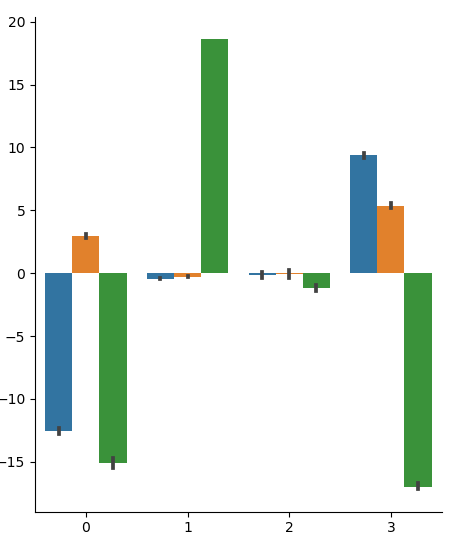
\includegraphics[width=0.9\linewidth]{AccelerometerResultsDay1.png}
\setlength\belowcaptionskip{-10pt}
\caption{Acceleration Barplot}
\label{Acceleration Factorplot}
\end{figure}

Cluster 1 can also be easy to interpret: The phone is constantly moving along its z axis (In the direction of the screen). If we take into account what we learned from the gyroscope, we know that the user of the phone has it in his pocket with the screen facing forward. This could mean that the user was travelling forward while standing, therefore the acceleration. The other two clusters are a lot more difficult to understand. It seems the phone is accelerating towards its left and down in cluster 0. In a similar fashion, the phone is moving to the right, up and contrary to its screen in cluster 3. Those kind of movements seem very wierd to us, and are then hard to define in terms of a person doing a clear activity. Another important thing is the number of points in each cluster. Clusters 1 and 3 have a lot less values than cluster 1. This seems to indicate that the person in day 1, according to our results, was accelerated forward most of the day.
\clearpage

\experiment{Interpreting the results: Acceleration, Day 2}

The most interesting thing we saw when analyzing the same sensors on a different day was the difference in the data. The features had the same relations, same correlation, but the data was completely different. This can also be seen in the results of the clustering (Figure \ref{Acceleration Factorplot 2}).

\begin{figure}[h]
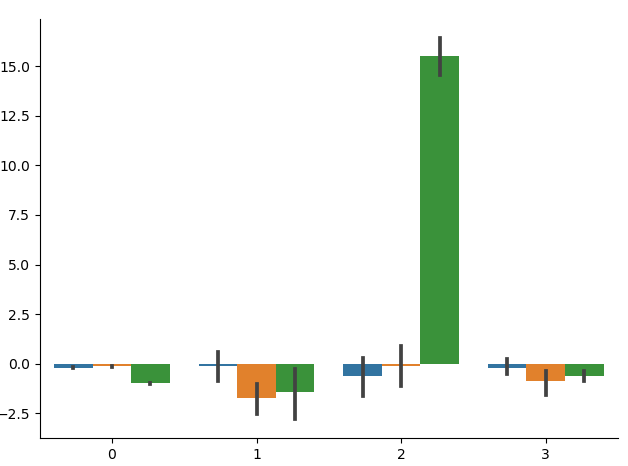
\includegraphics[width=0.9\linewidth]{AccelerometerResultsDay2.png}
\setlength\belowcaptionskip{-10pt}
\caption{Acceleration Barplot Day 2}
\label{Acceleration Factorplot 2}
\end{figure}

Two of the clusters we had are still present: Cluster 0 has all values close to 0, which means the phone is standing flat on a table. Cluster 0 has values close to 0 except for axis Z. This means, according to our interpretation, that the user is walking. The other 2 clusters are a lot different. On the one hand, most of their values have a very high variance, and also, their values are very scattered (One value can be of -3, while the next value, 15 seconds later, is 15). On the other hand, these 2 clusters (Cluster 1 and 3) have very little values. We are talking cluster 1 has 16 values out of more than 4000. These made us think that these clusters were bad results. Also, looking at the plot we obtained after applying k-means (\ref{K-Means plot 2 Selected} from the 30th of October), we could think that these clusters were created due to the supposition of k-means that the distribution of the data is globular, which in this case is not. Since our data seems a lot more dense in a particular area, we applied DBScan. Looking at the results of the DBScan, we can see that these 2 wierd clusters end up merging with cluster 0. This gives us a result of 2 clusters on this day: One where the phone was not being moved, and therefore not accelerated, and one where it was highly accelerated in the direction of the screen, presumably while moving (Like on Day 1).



\experiment{Interpreting the results: Outliers}

After we interpreted both the Accelerometer and the Gyroscope data the only task left is to interpret the outliers obtained through \textit{Local Outlier Factor}.
\\

First, we will interpret Day 1 of the Accelerometer, as we only have 28 data points we can easily see why they are outliers, all of them have zero or nearly to zero values in all columns except for one, the LinearAcceleration in the Z axis that corresponds to the vector that points to the sky.


We can interpret that the user in this specific day picked up the phone from a table few times throughout the day.
\\

Then, we will interpret Day 2 of the Accelerometer, this time we have a few more data points but we can also see why they're outliers, they all belong to cluster 0 so, as we said previously, the smartphone was standing on a table or another surface, the factor that makes them outliers is that the LinearAcceleration on one of the three axis is very high. So maybe the sensor suffered from a lot of environmental noise in that short period of time, or even the surface where the phone was lying in received a sudden movement/vibration.
\\

Finally, we are going to interpret the Gyroscope data, this time we also have few data points and, after exploring the data we dont see any special feature of the outliers, so we cannot give any interpretation of the data.


\end{document}